\documentclass[a4paper,12pt,twocolumn]{article}
\usepackage{graphicx}
\usepackage[margin=0.5in]{geometry}
\usepackage[cmex10]{amsmath}
\usepackage{array}
\usepackage{gensymb}
\usepackage{booktabs}
\title{Line Assignment}

\author{Ravi Sumanth Muppana- FWC22003}
\date{September 2022}
\providecommand{\norm}[1]{\left\lVert#1\right\rVert}
\providecommand{\abs}[1]{\left\vert#1\right\vert}
\let\vec\mathbf
\newcommand{\myvec}[1]{\ensuremath{\begin{pmatrix}#1\end{pmatrix}}}	
\newcommand{\mydet}[1]{\ensuremath{\begin{vmatrix}#1\end{vmatrix}}}
\providecommand{\brak}[1]{\ensuremath{\left((#1\right)}}
\begin{document}
\maketitle
\section{Problem:}
Show that if the diagonals of a quadrilateral bisect each other at right angles, then it is a rhombus
\maketitle
\section{Solution:}
\begin{figure}
	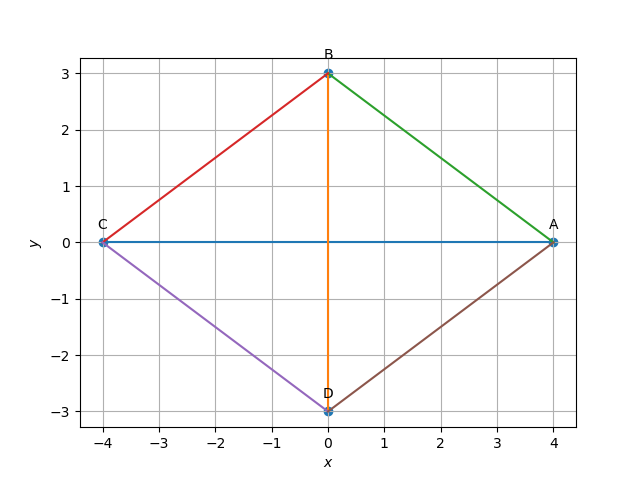
\includegraphics[width=\linewidth]{rhombus.png}
	\caption{Rhombus}
\end{figure}
\subsection{Theory:}
Given the diagonals bisect at right angles, we need to prove that all sides are equal, using vector algebra. Let us assume two vectors $\vec{A}$ and $\vec{B}$. The diagonals are the addition and subtraction of the two vectors:
\begin{align*}
&(\boldsymbol{A+B}), (\boldsymbol{B-A})
\end{align*}
\subsection{Mathematical Calculation:}
Let the two diagonals be $\boldsymbol{X}$, $\boldsymbol{Y}$. Since the diagonals are at right angle to each other,
\begin{align*}
&\boldsymbol{X}= \boldsymbol{A+B}\\
&\boldsymbol{Y}= \boldsymbol{B-A}\\
	&cos\theta = \frac{\boldsymbol{(A+B)}.\boldsymbol{(B-A)}}{||\boldsymbol{A+B}||.||\boldsymbol{B-A}||}\\
&cos90^{\circ} = 0 = (\boldsymbol{A+B}).(\boldsymbol{B-A})\\
&||\boldsymbol{B}||^2 - ||\boldsymbol{A}||^2 = 0\\
&||\boldsymbol{B}|| = ||\boldsymbol{A}||
\end{align*}
Hence, the two sides of the quadrilateral are equal. We need to prove the third side is also equal.
In triangle BOA and BOC;
\begin{align*}
&\boldsymbol{A} = \boldsymbol{X}- \boldsymbol{Y}\\
&\boldsymbol{D} =  \boldsymbol{-X}- \boldsymbol{Y}\\
\end{align*}
Now,
\begin{align*}
&||\boldsymbol{A}||^2 = ||\boldsymbol{X-Y}||^2\\
&||\boldsymbol{D}||^2 = ||\boldsymbol{-X-Y}||^2\\
&||\boldsymbol{A}||^2 = ||\boldsymbol{X}||^2 -2(\boldsymbol{X^T.Y}) +||\boldsymbol{Y}||^2\\
&||\boldsymbol{D}||^2 = ||\boldsymbol{X}||^2 +2(\boldsymbol{X^T.Y}) +||\boldsymbol{Y}||^2\\
\end{align*}
As the diagonals are perpendicular to each other, the terms $+2(\boldsymbol{X^T.Y})$ and $-2(\boldsymbol{X^T.Y})$ will be equal to zero. 
\begin{align*}
&||\boldsymbol{A}||^2 = ||\boldsymbol{X}||^2 + ||\boldsymbol{Y}||^2 \\
&||\boldsymbol{D}||^2 = ||\boldsymbol{X}||^2 + ||\boldsymbol{Y}||^2\\
&||\boldsymbol{A}|| = ||\boldsymbol{D} = ||\boldsymbol{B}||
\end{align*}
Hence, we have proved that the given quadrilateral is a parallelogram. A parallelogram with its diagonals as perpendicular bisectors is known as Rhombus.
\section{Construction:}
The construction of rhombus can be done using only two diagonals, taken as d1 and d2.
\begin{table}[h]
	\centering
\setlength\extrarowheight{2pt}
	\begin{tabular}{|c|c|c|}
		\hline
		\textbf{variable} & \textbf{length/point} & \textbf{Description}\\
		\hline
		d1 & 8 & length of diagonal 1\\
		\hline
		d2 & 6 & length of diagonal 2\\
		\hline
		A & (d1/2,0) & point A\\
		\hline                   
		B & (0,d2/0) & point B\\
		\hline
		C & (-d1/2,0) & point C\\
		\hline
		D & (0,-d2/2) & point D\\
		\hline
	\end{tabular}
\end{table}

\end{document}
